\documentclass[UTF8,a4paper,11pt]{article}

\usepackage{ctex} 
\usepackage{fancyhdr}
\usepackage{multicol} 
\usepackage{lastpage} 
\usepackage{geometry} 
\usepackage{hyperref}
\usepackage{titlesec} 
\usepackage{mathrsfs}
\usepackage{graphicx}
\usepackage{epstopdf}
\usepackage{ulem}
\usepackage{caption}
\usepackage{bm}%专门处理数学粗体的bm宏包
\usepackage{amsmath}
\usepackage[subfigure,AllowH]{graphfig} 

\geometry{left=3cm,right=3cm,top=2.5cm,bottom=2.5cm}
\renewcommand{\baselinestretch}{1.5}
\everymath{\displaystyle}


\title{\huge\heiti《信息论与编码》笔记}
\author{AlwaysLoveMisaka}
\date{\today}

\begin{document}
\maketitle
\thispagestyle{empty}
\begin{figure}[htbp]
\centering

\includegraphics[scale=0.27]{first.jpg}
\end{figure}
\clearpage

\tableofcontents
\setcounter{page}{1}
\pagenumbering{Roman}
\begin{figure}[htbp]
\centering

\includegraphics[scale=0.3]{p0.jpg}
\caption*{本笔记由天野阳菜\sout{(我的女朋友)}赞助}
\end{figure}
\clearpage

\setcounter{page}{1}
\pagenumbering{arabic}
\section{绪论}
\subsection{笔记说明}
这个笔记是基于《信息论与编码》(电子工业出版社)写的,我打算利用它梳理一下电磁场与电磁波的重点知识。由于我是边学边写的这个笔记,所以可能会有很多差错,敬请谅解。如果有同志发现笔记的错误,可以通过QQ联系(本人账号:876563962)。另外,此手册也不能作为考点参考,因为我也不知道考试到底考啥。

\subsection{信息的定义}
1948年,著名数学家,通信工程奠基人香农发表了论文《通信的数学理论》,这标志着信息论的诞生,香农认为信息是\textbf{不确定性的减少量},而不确定性与概率负相关,因此,可以使用概率论的数学工具描述信息。
\begin{figure}[htbp]
\centering
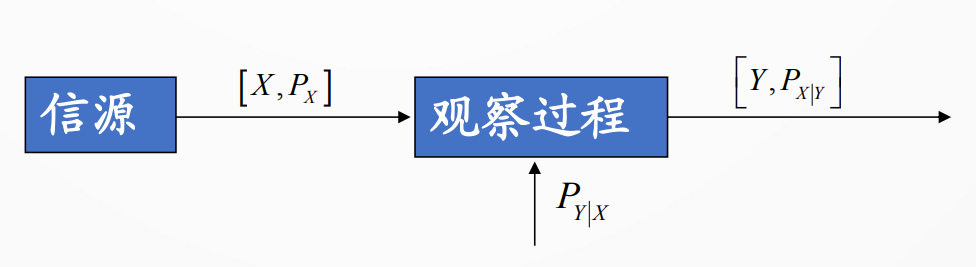
\includegraphics[scale=0.6]{p1.png}
\caption{非理想观察模型}
\end{figure}

我们可以将通信过程视为一个非理想的观察过程,如图1,信源为$X$,经观察后输出为$Y$。$P(X)$称为先验概率,$P(X|Y)$称为后验概率。由于信息是不确定性的减少量,因此我们可以得到一个定性等式:信息$=$先验不确定性$-$后验不确定性。

这个等式是一个粗略的描述,我们在以后的章节会进行细化。

$P(X|Y)$指在事件$X$发生的前提下,$Y$发生的概率,也叫条件概率。条件概率的基本性质如下:
\begin{itemize}
\item 乘法性质:$P(B|A)P(A)=P(AB)$
\item 独立性:$P(A|B)=P(A)$的充要条件是$A$和$B$相互独立
\item 贝叶斯定理:$P(B|A)=\frac{P(A|B)P(B)}{P(A)}$
\end{itemize}

\subsection{课程的主要内容}
本课程主要解决的问题在于找到信息传输过程中的共同规律,以提高信息传输的可靠性、有效性、保密性和认证性,以达到信息传输系统最优化。

图二是基本的通信系统模型,信源编译码器的作用是用二进制序列来表示信源输出,信道译码器的作用是实现无差错通信。书的第二章主要讨论了信源和熵,第三章信道的数学模型和信道容量,第四章和第五章分别讨论了信源编码和信道编码,前五章是期末考试的范围。
\begin{figure}[htbp]
\centering
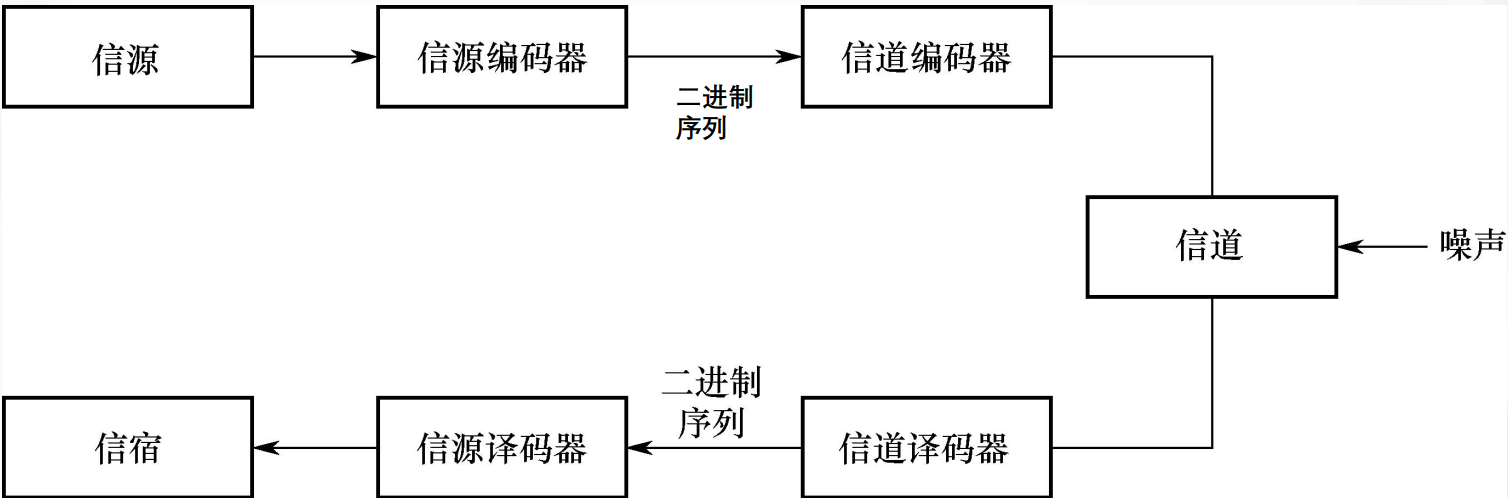
\includegraphics[scale=0.45]{p2.png}
\caption{通信系统模型}
\end{figure}

\section{信源与熵}
\subsection{香农熵}
在通信系统中,信源可以看作一类随机变量序列,比如说天气预报信息的发送,就可以看作以下的这种随机变量:$X=\{x_1=sunny,x_2=cloudy,x_3=snowy,x_4=rainy\}$。

有记忆信源和无记忆信源是信息理论中的两个重要概念,它们描述了信源生成信息的特性。无记忆信源是指每个符号的产生都是相互独立的,即每个符号的产生概率只取决于该符号本身,而与之前或之后的符号无关。例如,投掷一枚硬币或者掷一颗骰子就是一个无记忆信源。相反,有记忆信源则是指符号的产生概率依赖于之前产生的符号序列。在有记忆信源中,后面的符号产生概率取决于前面的符号序列,而不仅仅是当前符号。例如,一个文本序列就是一个有记忆信源,因为每个单词的出现概率往往会受到前面的单词和上下文的影响。因此,有记忆信源和无记忆信源的主要区别在于是否考虑先前生成的符号对当前符号的产生概率的影响。在信息传输和压缩等领域中,这个区别非常重要,因为它们需要使用不同的编码方案来表示不同类型的信源。在以后的讨论中,讨论的信源主要是离散无记忆信源(DMS)。

在19世纪,熵是一个热力学的概念,它用来描述一个热力学系统混乱程度的概念,是系统热力学状态的一个函数,一个系统的熵越大,说明它的混乱程度越高。

香农将熵的概念从热力学引入到信息理论中,他提出了\textbf{香农熵}的概念,来表示信源的“混乱程度”。假设有一事件集合$X\in \{x_1,x_2,\cdots,x_n\}$,任一事件发生的概率分别为 $\{p_1,p_2,\cdots,p_n\}$,则这个事件(信源)的香农熵可以表示为:
\begin{equation}
H(p_1,p_2,\cdots,p_n)=-\sum_{k=1}^n p_k{\rm log}p_k
\end{equation}

可以看到,上述定义的对数没有底,实际上,这个对数的底是任意的,都不会影响到香农熵的性质。在下文中如果不加说明,那么就默认取2为底。为了度量某一单独事件$x_k$的信息量,我们引入\textbf{自信息量}:
\begin{equation}
I(x_k)=-{\rm log}P(x_k)
\end{equation}

可以看出,香农熵就是自信息量的加权平均数,即一组事件的平均不确定性度量。不确定性的单位和对数的底的选取有关,若对数的底为2,则称为比特,若对数的底为e,则称为奈特,若对数的底为10,则称为迪特。

香农熵有以下特性:
\begin{itemize}
\item 可扩展性:
\begin{equation}
H(p_1,p_2,\cdots,p_n)=H(p_1,p_2,\cdots,p_n,0)
\end{equation}

\item 确定性:当且仅当某个$p_k$为1时,$H(X)=0$。
\item 上凸性:$H(p_1,p_2,\cdots,p_n)$是上凸函数。
\item 极值性:
\begin{equation}
H(p_1,p_2,\cdots,p_n)\le \log_{2}{n}
\end{equation}
\end{itemize}

信源的\textbf{信息速率}$R_t$是信源单位时间内发出的平均信息量,若信源平均$t_s$秒发出一个符号,则有
\begin{equation}
R_t=\frac{H(X)}{t_s}
\end{equation}

\textbf{信息含量效率}$\eta$有如下定义:
\begin{equation}
\eta=\frac{H(X)}{H_{max}(X)}=\frac{H(X)}{\log_{2}{n}}
\end{equation}

另外,我们定义
\begin{equation}
\gamma=1-\eta
\end{equation}
为\textbf{信息的相对冗余度},表示信源含无效成分的程度。

\subsection{联合熵与条件熵}
在上述的讨论中,我们使用一维的概率集合来表示信源和信源的香农熵,如果信源是二维的,那么就需要使用联合概率分布来表示其香农熵。联合分布的随机变量$XY$的信息度量被称为\textbf{联合熵},记为:
\begin{equation}
H(XY)=-\sum_{k=1}^n\sum_{j=1}^mP(x_k,y_j)\log_{2}{P(x_k,y_j)}
\end{equation}

当$Y$已知时,$X$的平均不确定性为:
\begin{equation}
H(X|Y)=-\sum_{k=1}^n\sum_{j=1}^mP(x_k,y_j)\log_{2}{P(x_k|y_j)}
\end{equation}

上式被称为$Y$是已知条件下$X$的\textbf{条件熵}。可以证明:
\begin{equation}
H(XY)=H(X)+H(Y|X)=H(Y)+H(X|Y)
\end{equation}

如果$X$和$Y$相互独立,则有
\begin{equation}
\begin{cases}
H(XY)=H(X)+H(Y) \\
H(X|Y)=H(X) \\
\end{cases}
\end{equation}

\subsection{平均互信息量}
我们引入\textbf{平均互信息量}的概念,用来描述香农对“信息”的定义。随机变量$X$和$Y$的互信息量为:
\begin{equation}
\begin{aligned}
I(X;Y)&=H(X)+H(Y)-H(XY) \\
&=H(Y)-H(Y|X) \\
&=H(X)-H(X|Y)
\end{aligned}
\end{equation}

而单一符号的互信息量为:
\begin{equation}
I(x_k;y_j)=I(x_k)-I(x_k|y_j)
\end{equation}

由定义可知,若$X$和$Y$互相独立,则$I(X;Y)=0$。

平均互信息量有以下基本性质
\begin{itemize}
\item 互易性:$I(X;Y)=I(Y;X)$
\item 非负性:$I(X;Y)\ge 0$。由此可以得出:
\begin{equation}
H(X)\ge H(X|Y)
\end{equation}

\item 有界性:
\begin{equation}
I(X;Y)\le H(X)
\end{equation}

也就是说,从$Y$得到的关于$X$的信息,不会多于$X$自身的实在信息
\end{itemize}

\subsection{连续信源的信息熵}
如果$X$是连续随机变量,其概率密度函数由$f_X(x)$描述,我们将连续随机变量$X$的\textbf{微分熵}记为:
\begin{equation}
h(X)=\int_{-\infty}^{\infty} {f_X(x)\log_{2}{f_X(x)}} \,{\rm d}x
\end{equation}

微分熵具有如下性质:
\begin{itemize}
\item 不满足非负性
\item 可加性(香农熵也满足),即
\begin{equation}
\begin{cases}
h(XY)=h(X)+h(Y|X)=h(Y)+h(X|Y) \\
h(X)\ge h(X|Y) \\
h(Y)\ge h(Y|X) \\
h(XY)\le h(X)+h(Y) \\
\end{cases}
\end{equation}

当且仅当$X$和$Y$相互独立时,等号成立。
\end{itemize}

微分熵的极大化问题是指,在给定某些约束条件下,求一个连续随机变量的概率密度函数,使得该概率密度函数对应的微分熵最大。下面我们讨论两种情况。

\begin{enumerate}

\item \textbf{幅值受限}

所谓幅值受限,指的是$f_X(x)$只在某个连续的区间内不为0。可以证明,在幅值受限条件下,随机变量服从均匀分布时,微分熵最大。设$X$取值受限于$[a,b]$,那么它的最大微分熵为$\log_{2}{(b-a)}$。

\item \textbf{方差受限}

可以证明,均值一定是,在方差受限条件下,随机变量服从正态分布时,微分熵最大。设$X$的均值为$\mu$,方差受限为$\sigma^2$时,最大微分熵为$\log_{2}{\sqrt{2\pi e\sigma^2}}$。
\end{enumerate}

\section{信道及其容量}
\subsection{信道的基本参数}
离散无记忆信道(DMC)是指在一定时间内,接收端和发送端之间的通信信道不会发生任何变化,且每次发送的符号只受到当前发送符号的影响,而与之前发送的符号和接收到的符号无关。若不进行特别说明,本章讨论的信道都是DMC。

我们假设在离散无记忆信道中,我们假设输入的随机变量为$X$,它取值于输入符号集$A\in \{a_1,a_2,\cdots,a_r\}$,输出的随机变量为$Y$,它取值于输出符号集$B\in \{b_1,b_2,\cdots,b_s\}$。构成的数学模型如图1。条件概率$P(b_j|a_i)$描述了输入至输出状态转移的统计特性,也称转移概率。显然一共有$r\cdot s$个转移概率,我们将其排成一个$r\times s$的矩阵,称为\textbf{转移矩阵},记为$\bm{P_{Y|X}}$。
\begin{equation}
\bm{P_{Y|X}}=
\begin{bmatrix}
P(b_1|a_1)&P(b_2|a_1)&\cdots&P(b_s|a_1)\\
P(b_1|a_2)&P(b_2|a_2)&\cdots&P(b_s|a_2)\\
\vdots&\vdots&\ddots&\vdots\\
P(b_1|a_r)&P(b_2|a_r)&\cdots&P(b_s|a_r)\\
\end{bmatrix}
\end{equation}

显然有:
\begin{equation}
\sum_{j=1}^sP(b_j|a_i)=1
\end{equation}

我们也可以用\textbf{信道线图}来表示DMC模型,图3是二进制对称信道(BSC)的线图,其他各种信道的线图可参考教材p48。
\begin{figure}[htbp]
\centering
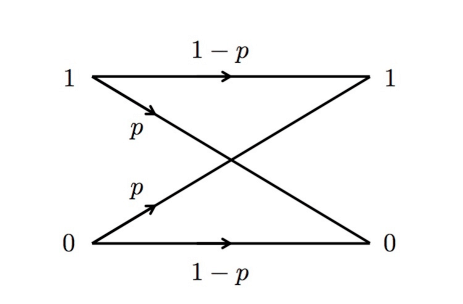
\includegraphics[scale=0.45]{p3.png}
\caption{二进制对称信道}
\end{figure}

由第二章的知识可知:
\begin{equation}
\begin{cases}
I(X;Y)\le H(X) \\
I(X;Y)\le H(Y) \\
\end{cases}
\end{equation}

$I(X;Y)$可以看作$Y$从$X$得到的平均信息量,由于干扰的影响,来自输入的部分信息在传输过程中丢失了,损失的部分就是$H(X|Y)$。因此,我们通常把$H(X|Y)$称为信道${X,P_{Y|X},Y}$的\textbf{疑义度}或\textbf{损失熵}。损失熵为0的信道称为\textbf{无损信道}。

从另一个角度来说,$H(Y)$代表输出的所有信息,其中有用信息$I(X;Y)$只占其中一部分,那么两者的差值$H(Y|X)$可以视为由噪声引入的无用信息。因此,我们通常把$H(Y|X)$称为信道${X,P_{Y|X},Y}$的\textbf{散布度}或\textbf{噪声熵}。噪声熵为0的信道称为\textbf{确定信道}。

\subsection{计算DMC的信道容量}
每个给定的信道都存在一个最大的信息率,这就是该信道的\textbf{信道容量},即
\begin{equation}
C=I(X;Y)_{max}
\end{equation}

使得给定信道的$I(X;Y)$达到最大值的输入分布,称为\textbf{最佳输入分布},记为$\bm{P^*_X}$。

实际上,计算一般信道的信道容量是个很困难的问题,我们只能从一些特殊的情况入手。首先我们讨论无噪信道的信道容量求法,无噪信道是无损信道、确定信道和无损确定信道的统称。下面举三个例子说明。

\begin{enumerate}
\item \textbf{无损信道}

首先设定一个无损信道的转移矩阵:
\begin{equation}
\notag
\bm{P_{Y|X}}=
\begin{bmatrix}
0.5&0.5&0&0&0&0\\
0&0&0.2&0.4&0.4&0\\
0&0&0&0&0&1\\
\end{bmatrix}
\end{equation}

可以看出,无损信道每列只有一个非零元素。可以证明,当输入为等概率分布时,$I(X;Y)$得到最大值,因此
\begin{equation}
\notag
C=I(X;Y)_{max}=H(X)_{max}=\log_{2}{3}
\end{equation}

\item \textbf{确定信道}

一个典型的确定信道转移矩阵如下:
\begin{equation}
\notag
\bm{P_{Y|X}}=
\begin{bmatrix}
1&0\\
1&0\\
0&1\\
0&1\\
0&1\\
\end{bmatrix}
\end{equation}

同理:
\begin{equation}
\notag
C=I(X;Y)_{max}=H(Y)_{max}=\log_{2}{2}=1
\end{equation}

\item \textbf{无损确定信道}

损失熵和噪声熵均为0的信道被称为\textbf{无损确定信道},其转移矩阵一定是一个单位阵,即:
\begin{equation}
\bm{P_{Y|X}}=
\begin{bmatrix}
1&0&\cdots&0\\
0&1&\cdots&0\\
\vdots&\vdots&\ddots&\vdots\\
0&0&\cdots&1\\
\end{bmatrix}
\end{equation}

显然
\begin{equation}
C=I(X;Y)_{max}=\log_{2}{r}
\end{equation}
其中$r$是矩阵的长。
\end{enumerate}

除了无噪信道,\textbf{对称信道}的信道容量也是可以计算的。对称信道是一种特殊的通信信道,其特点是在两个方向上传输信息时具有相同的特性和信道传输概率。也就是说,无论信息是从发送方到接收方还是从接收方到发送方传输,信道的特性和传输概率都是相同的。

一个典型的\textbf{离散对称信道}的转移矩阵如下:
\begin{equation}
\notag
\bm{P_{Y|X}}=
\begin{bmatrix}
0.3&0.3&0.2&0.2\\
0.2&0.2&0.3&0.3\\
\end{bmatrix}
\end{equation}

可以看出,若一个信道的转移矩阵每行的元素一样,且每列的元素也一样,这种矩阵被称为\textbf{行列排列阵}。


可以证明,对于对称DMC,
\begin{equation}
C=\log_{2}{s}-H(X')
\end{equation}

其中,$X'$是转移矩阵任意一行元素的集合。

我们可以计算出上述例子的信道容量:
可以证明,对于对称DMC,当输入等概率时达到信道容量:
\begin{equation}
\notag
C=\log_{2}{s}-H(X')=2-1.971=0.029
\end{equation}

如果把对称性条件减弱一点,那么可以给出准对称信道的定义。若某个信道的转移矩阵可被划分为若干互不相交的子阵,每个子阵都是行列排列阵。我们举一个例子来说明,二进制删除信道(BEC)如图4所示。
\begin{figure}[htbp]
\centering
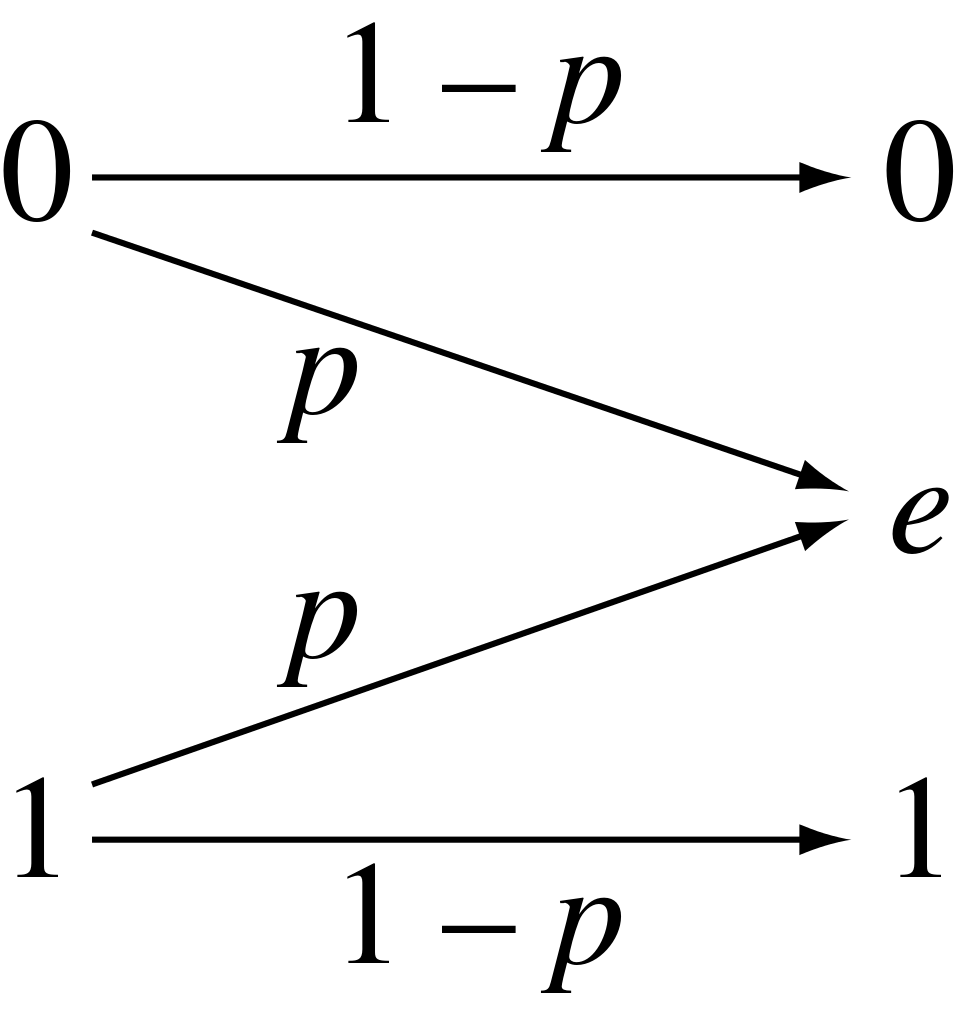
\includegraphics[scale=0.15]{p4.png}
\caption{二进制删除信道}
\end{figure}

我们可以写出它的转移矩阵:
\begin{equation}
\notag
\bm{P_{Y|X}}=
\begin{bmatrix}
1-p&0&p\\
0&1-p&p\\
\end{bmatrix}
\end{equation}

然后我们可以将其拆分成两个子阵:
\begin{equation}
\notag
\begin{bmatrix}
1-p&0\\
0&1-p\\
\end{bmatrix}
\quad
\begin{bmatrix}
p\\
p\\
\end{bmatrix}
\end{equation}

显然,这两个子阵都是行列排列阵。因此,BEC是一个准对称矩阵。可以证明,如果将准对称DMC的$\bm{P_{Y|X}}$分为$n$个行列排列子阵$\{\bm{Q_1},\cdots,\bm{Q_n}\}$,则有
\begin{equation}
C=-\sum_{k=1}^n\frac{s_kM_k}{r}\log_{2}{\frac{M_k}{r}}-H(X')
\end{equation}

上式中,$r$是$\bm{P_{Y|X}}$的行数,$s_k$是,$\bm{Q_k}$的列数,$M_k$是,$\bm{Q_k}$的任意一列元素之和,$X'$是转移矩阵任意一行元素的集合。另外,准对称信道也是输入等概率时达到信道容量。因此我们可以求BEC的信道容量:
\begin{equation}
\notag
\begin{aligned}
C&=-\frac{2(1-p)}{2}\log_{2}{\frac{1-p}{2}}-\frac{2p}{2}\log_{2}{\frac{2p}{2}}+(1-p)\log_{2}{(1-p)}+p\log_{2}{p}\\
&=(1-p)\log_{2}{2}\\
&=1-p
\end{aligned}
\end{equation}

\subsection{连续信道及其信道容量}
\textbf{连续信道}是时间离散,幅值连续信道的简称。与离散信道类似,连续信道的信道容量也有(21)式的性质。在实际应用中,信道输入信号的平均功率$E(X^2)$总是限定在某个范围内,因此,连续信道在平均输入功率受限时的信道容量为:
\begin{equation}
C=max\{I(X;Y),E(X^2)\le P_S\}
\end{equation}

和DMC一样,求解一般连续信道的信道容量非常困难,只有一些特殊的连续信道才能推出信道容量的表达式。下面我们介绍\textbf{加性噪声信道}的信道容量计算方法。

如果信道的输入$X$、输出$Y$和噪声$Z$满足
\begin{equation}
Y=X+Z
\end{equation}

且$X$和$Z$无关,那么该信道就是加性噪声信道。

假设加性噪声$Z$服从均值为0,方差为$\sigma^2_Z$的高斯分布,那么这时其方差就有明确的物理意义,它等于$Z$的平均功率$P_N$:
\begin{equation}
\sigma^2_Z=E(Z^2)=P_N
\end{equation}

可以证明,加性高斯噪声信道的信道容量为
\begin{equation}
C(P_S)=\frac{1}{2}\log_{2}{(1+\frac{P_S}{P_N})}
\end{equation}

在加性高斯噪声信道中传输信息时,高斯分布的输入信号是最有效的,反过来,若输入信号服从高斯分布,高斯噪声是最有害的。而对于一般的无记忆加性噪声,我们可以给出其上下界:
\begin{equation}
\frac{1}{2}\log_{2}{(1+\frac{P_S}{P_N})}\le C(P_S)\le\frac{1}{2}\log_{2}{\frac{P_S+P_N}{P_e}}
\end{equation}

式中,
\begin{equation}
P_e=\frac{1}{2\pi e}e^{2h(Z)}
\end{equation}

\subsection{波形信道及其信道容量}
\textbf{波形信道}是指取值连续,时间也连续的信道,也被称为\text{模拟信道}。我们这里只讨论带限、加性高斯白噪声信道。

白噪声的的功率谱密度是均匀的,如果白噪声的频带限制$B$,其功率谱密度为:
\begin{equation}
P_Z(f)=\frac{N_0}{2}\quad(-B\le f\le B)
\end{equation}

可以证明,带限、加性高斯白噪声信道的信道容量为:
\begin{equation}
C(P_S)=B\log_{2}{(1+\frac{P_S}{N_0B})}\quad bit/s
\end{equation}

这就是著名的\text{香农信道容量公式},根据这个公式,我们可以得到两种扩大信道容量的方法:
\begin{itemize}
\item 扩大频带,这种方法在空间通信中很常用。但是用扩频法扩大的信道容量是有限的,因为

\begin{equation}
\lim_{B \to \infty}C(P_S)\approx 1.44\frac{P_S}{N_0}
\end{equation}

\item 提高信噪比,但是这种方法也有局限性。若把$P_S$当作变量,那么$C'(P_S)$是一个单调递减趋于0的函数,这意味着当$P_S$增大到一定程度后,再增加很多,$C(P_S)$的增长幅度也很小。
\end{itemize}

我们使用\textbf{信道相对剩余度}来描述信源与信道的信息匹配程度:
\begin{equation}
\text{信道相对剩余度}=\frac{C-I(X;Y)}{C}
\end{equation}

别问我为什么信道相对剩余度没有数学符号,我也不知道。剩余度小,说明信源和信道匹配度高,信道的信息传递得到充分利用。

\section{无失真信源编码}
\subsection{信源编码的基本概念}
无失真信源编码是一种信息编码技术,其目的是将源数据压缩成更小的数据集,同时保留原始数据的所有信息,不产生任何损失。

\begin{figure}[htbp]
\centering
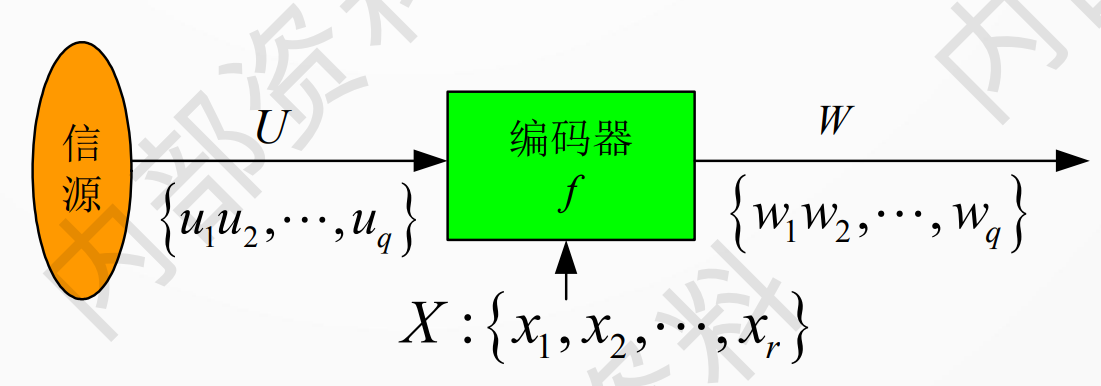
\includegraphics[scale=0.45]{p5.png}
\caption{信源编码器示意图}
\end{figure}

信源编码器如图5所示,下面介绍一下部分信源编码的基本概念:

\begin{itemize}
\item \textbf{码元}

信道能够传送的符号$x_i$被称为码元。

\item \textbf{码字}

码元序列$w_i$被称为码字。

\item \textbf{定长编码}、\textbf{变长编码}

若所有的码字均有相同的码长$l$,则称$f$为定长编码,否则称为变长编码。

\item \textbf{平均码长}

对码$W$中所有码字的码长求统计平均,得平均码长$\overline{l}$:
\begin{equation}
\overline{l}=\sum_{i=1}^q P(w_i)l_i
\end{equation}

\item \textbf{编码效率}

为了衡量编码效果,定义编码后的实际信息率和编码后的最大信息率之比就是编码效率:
\begin{equation}
\eta_c=\frac{H(U)}{\overline{l}\log_{2}{r}}
\end{equation}

式中,$r$为编码使用的进制。

\item \textbf{编码冗余度}

编码冗余度表示编码中无用信息的占比:
\begin{equation}
\gamma_c=1-\eta_c
\end{equation}
\end{itemize}

\subsection{编码的唯一可译性}
我们可以通过编码的各种特征,对编码进行分类,下面举几个基本的编码分类。
\begin{figure}[htbp]
\centering
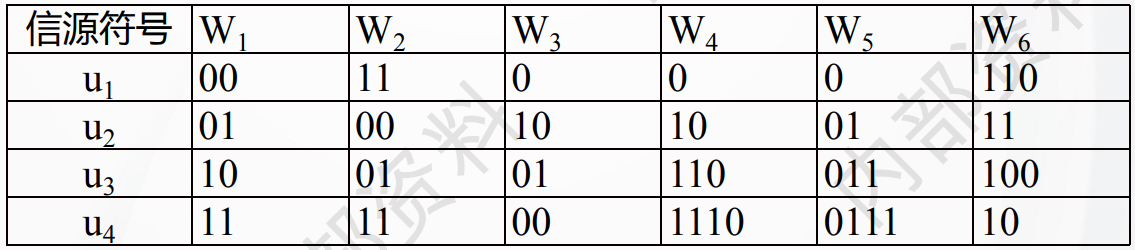
\includegraphics[scale=0.45]{p6.png}
\caption{编码举例}
\end{figure}

\begin{figure}[htbp]
\centering
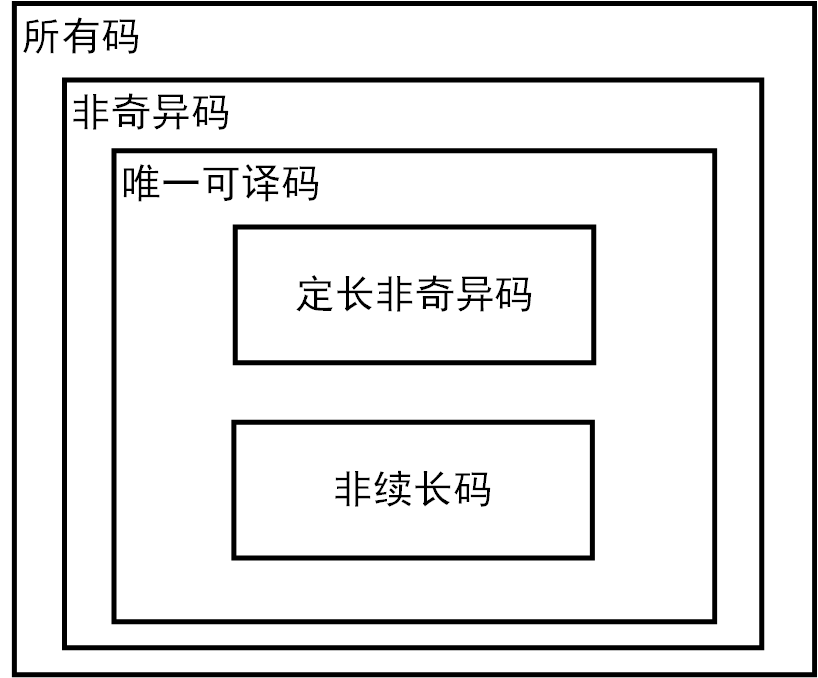
\includegraphics[scale=0.45]{p7.png}
\caption{各种码的关系}
\end{figure}

\begin{itemize}
\item \textbf{唯一可译码}与\textbf{非唯一可译码}

唯一可译码(UDC)是一种编码方式,其特点是能够通过解码得到唯一的原始消息。在信息传输中,为了节省带宽和提高传输效率,常常需要对消息进行编码,将其转换为一组数字或符号,然后再进行传输。然而,在编码过程中,可能会出现多个编码对应同一个原始消息的情况,这被称为编码不唯一性。如果编码不唯一,那么在解码的过程中,就无法确定原始消息是哪个,这会导致信息传输出现错误或丢失。唯一可译码就是为了解决编码不唯一性而设计的一种编码方式。它要求在任何情况下,都可以通过解码得到唯一的原始消息,避免了信息传输中出现错误或丢失的情况。如果不满足上述条件,则是非唯一可译码。

\item \textbf{奇异码}与\textbf{非奇异码}

如图6中的$W_2$,它有相同的码字,这种码被称为奇异码,否则称为非奇异码。奇异码一定不是UDC,定长非奇异码一定是UDC。

\item \textbf{续长码}与\textbf{非续长码}

观察$W_4$可以发现,它的每个符号的编码都是唯一的且不是另一个符号编码的前缀。这意味着我们可以根据编码的前缀来确定一个符号的编码,而无需查看编码的完整序列,这种编码被称为非续长码。而不满足这种特性的则称为非续长码,如$W_5$。

\end{itemize}

各种码的关系如图7所示。可以证明,对于$r$进制非续长码,一定满足\textbf{克拉夫特不等式}:
\begin{equation}
\sum_{i=1}^q r^{-l_i}\le 1
\end{equation}

反过来,若上式成立,就一定能构造一个$r$进制非续长码。克拉夫特不等式还是存在UDC的充要条件,对于任意一个$r$进制UDC,必须满足(39)。

\subsection{无失真定长/变长编码定理}
前面讨论编码时,都是对信源输出的单个符号进行编码的。现在考虑更一般的情况,即对信源输出符号序列进行编码。
可以证明,用$r$元符号表对离散无记忆信源$U$的$N$长符号序列进行定长编码,$N$长符号序列对应的码长是$l_N$,如果对于任意的正数$\epsilon$,当$N$足够大时,恒有
\begin{equation}
\frac{l_N}{N}\ge\frac{H(U)+\epsilon}{\log_{2}{r}}
\end{equation}
那么就能几乎做到无失真编码,随着$N$的增大,译码差错率趋于0。反之,若
\begin{equation}
\frac{l_N}{N}\le\frac{H(U)-2\epsilon}{\log_{2}{r}}
\end{equation}
则不可能做到无失真编码,随着$N$的增大,译码差错率趋于1。

我也不知道(41)式$\epsilon$的系数2是哪来的\sout{(我的女朋友天野阳菜也不知道)},知道的同志可以联系我一下。

可以证明,定长编码的效率为:
\begin{equation}
\eta_c=\frac{NH(U)}{l_N\log_{2}{r}}
\end{equation}

变长编码也有类似于式(40)(41)的定理。可以证明,用$r$元符号表对离散无记忆信源$U$的$N$长符号序列进行定长编码,$N$长符号序列对应的平均码长是$\overline{l_N}$,那么要做到无失真编码,平均码长必须满足
\begin{equation}
\frac{\overline{l_N}}{N}\ge H_r(U)
\end{equation}

另一方面,一定存在唯一可译码,满足
\begin{equation}
\frac{\overline{l_N}}{N}\le H_r(U)+\frac{1}{N}
\end{equation}

式(43)(44)被称为\textbf{香农第一编码定理},它给出了信源有效编码的基本界限。

\subsection{三种经典无失真信源编码方法}
变长编码采用非续长码,力求平均码长最小,此时编码效率最高,信源的冗余得到了最大程度的压缩。对给定的信源,使平均码长最小的编码方法称为\textbf{最佳编码}。下面,我们举一例来解释三种经典的无失真信源编码方法。现有如下DMS:
\begin{equation}
\notag
\begin{bmatrix}
U\\ 
P_U\\ 
\end{bmatrix}
=
\begin{bmatrix}
u_1&u_2&u_3&u_4&u_5&u_6&u_7\\ 
0.35&0.3&0.2&0.1&0.04&0.005&0.005\\ 
\end{bmatrix}
\end{equation}

易求得
\begin{equation}
\notag
H(U)=2.11
\end{equation}

我们先用定长非奇异码$U$进行编码,如图8。
\begin{figure}[htbp]
\centering
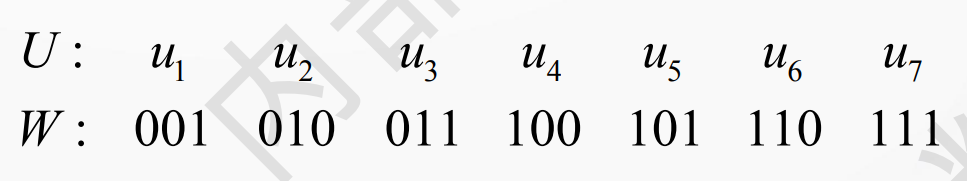
\includegraphics[scale=0.45]{p8.png}
\caption{定长非奇异码示例}
\end{figure}

因此$\overline{l}=3$,且
\begin{equation}
\notag
\eta_c=\frac{2.11}{3\cdot\log_{2}{2}}=70.33\%
\end{equation}

\textbf{霍夫曼编码}是一种无损数据压缩算法,它将频率高的字符用较短的编码表示,频率低的字符用较长的编码表示。

以下是二进制霍夫曼编码的具体过程:
\begin{enumerate}
\item \textbf{统计字符频率}

首先需要统计待压缩数据中每个字符出现的频率。将字符及其频率记录在一个字符频率表中。

\item \textbf{构建霍夫曼树}

将字符频率表中的每个字符看作一个节点,然后按照它们的频率构建一棵二叉树,构建过程中频率低的字符放在树的下层,频率高的字符放在树的上层,构建的过程中需要不断合并频率最小的两个节点,直到只剩下一个节点。

\item \textbf{分配编码}

在霍夫曼树构建完成后,从根节点开始遍历树,当走到一个字符节点时,记录从根节点到该节点的路径,将路径上的0和1分别对应编码的0和1,这样就得到了每个字符对应的编码。
\end{enumerate}

按照上述原则,我们可以对$U$进行霍夫曼编码,如图9。
\begin{figure}[htbp]
\centering
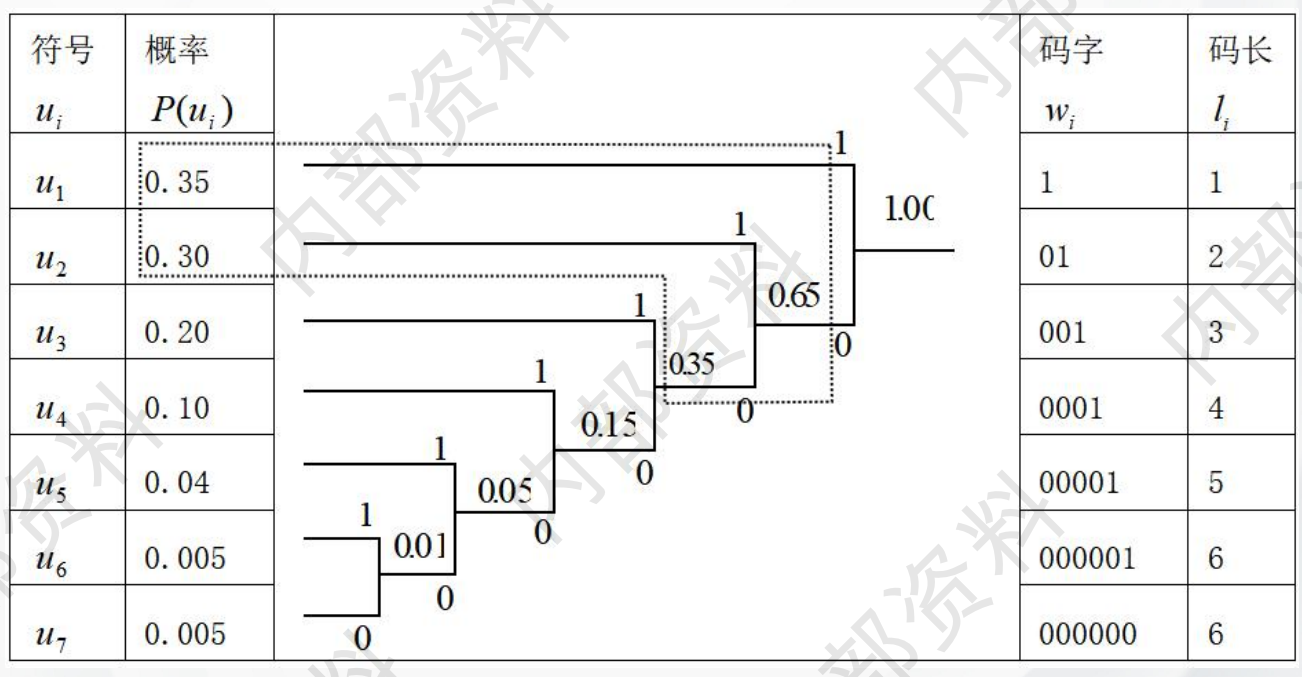
\includegraphics[scale=0.45]{p9.png}
\caption{霍夫曼编码示例}
\end{figure}

此时我们可以计算出:
\begin{equation}
\notag
\eta_c=\frac{2.11}{2.21\cdot\log_{2}{2}}=95.48\%
\end{equation}

可以看出,霍夫曼编码可以取得较好的冗余压缩效果,使输出码元概率均匀化。\textbf{费诺编码}和霍夫曼编码相似,都是非续长码的生成方法。费诺编码的步骤如下:

\begin{enumerate}
\item 确定需要编码的字符集和它们出现的频率。在这个步骤中,需要计算每个字符出现的频率,并按照频率从高到低进行排序。

\item 将字符集一分为二,使得两个子集中字符的出现频率之和尽可能接近。这个步骤的目的是将编码的负担尽可能平均地分摊到每个字符上。

\item 对于每个子集,递归地进行步骤2,直到每个子集中只包含一个字符为止。

\item 对于每个字符,给它们分配一个编码,使得编码满足以下条件:

(1)编码不是任何其他编码的前缀。

(2)对于任何一个字符,它的编码是由根节点到该字符节点的路径上的左右方向决定的。
\end{enumerate}

所以,费诺编码不一定严格按照概率匹配编码,因而不一定是最佳码。

按照上述原则,我们可以对$U$进行费诺编码,如图10。

\begin{figure}[htbp]
\centering
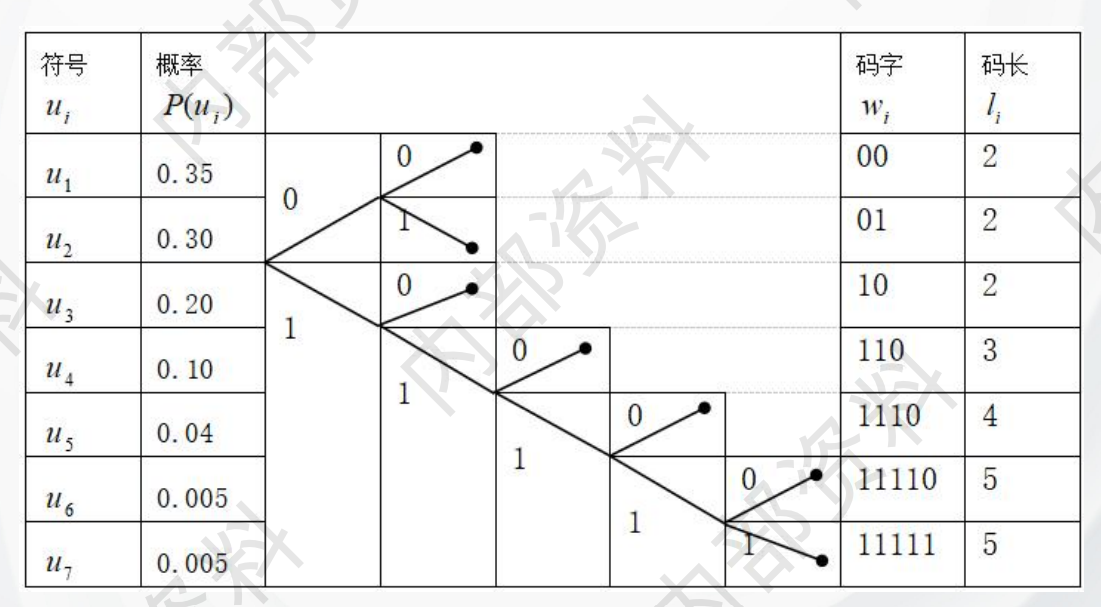
\includegraphics[scale=0.45]{p10.png}
\caption{费诺编码示例}
\end{figure}

此时我们可以计算出:
\begin{equation}
\notag
\eta_c=\frac{2.11}{2.21\cdot\log_{2}{2}}=95.48\%
\end{equation}

在这种情况下霍夫曼编码和费诺编码的效率是一样的,但是大多数情况费诺编码的效率会偏低。

\begin{figure}[htbp]
\centering
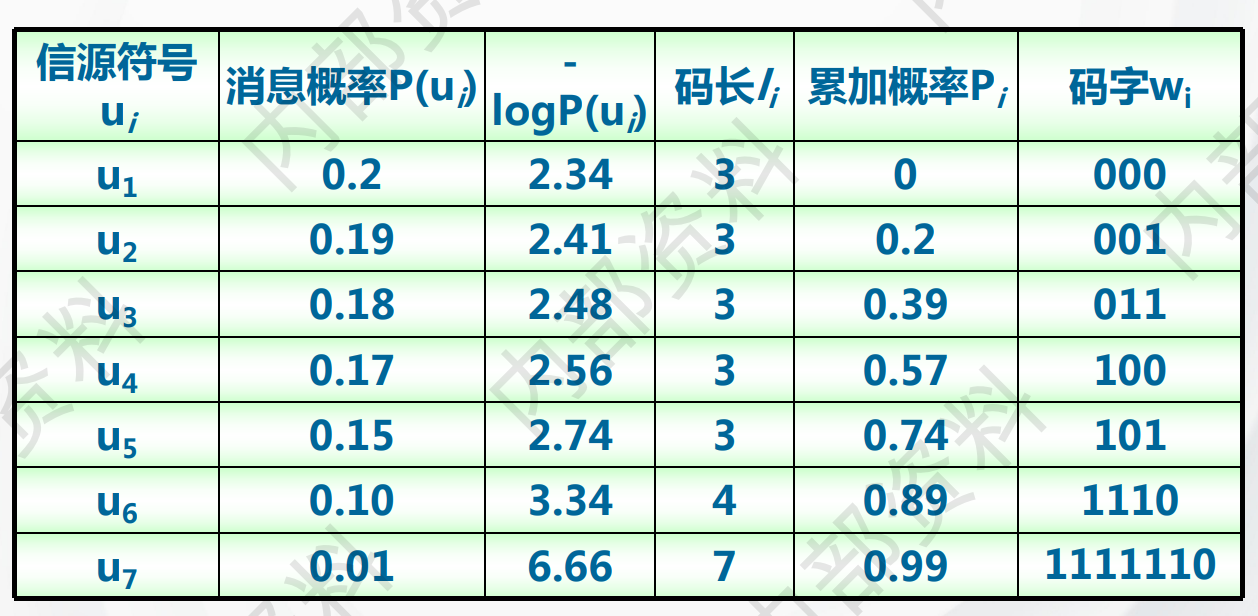
\includegraphics[scale=0.45]{p11.png}
\caption{香农编码示例}
\end{figure}

\textbf{香农编码}是另一种构造非续长码的方法,它的编码步骤是:
\begin{enumerate}
\item 将信源符号按概率从大到小降序排列

\item 求每个符号对应的码长,并取整,计算方法如下:
\begin{equation}
-\log_{2}{P(U_i)}\le l_i\le -\log_{2}{P(U_i)}+1
\end{equation}

\item 将累加概率小数点后的$l_i$位作为码字

\end{enumerate}

按照上述原则,我们可以对$U$进行香农编码,如图11。此时我们可以计算出:
\begin{equation}
\notag
\eta_c=\frac{2.11}{3.14\cdot\log_{2}{2}}=83.1\%
\end{equation}

比较可知,霍夫曼编码效率最高,费诺编码次之,香农编码效率最低。因此,香农编码的实用价值不大。但是它有深远的理论意义,因为使用香农编码时,当序列长度逼近无穷大时,平均码长会趋近于信源的熵。


\section{信道纠错编码}

下面我们将用一个例子解释一下\textbf{平均差错率}。

\textbf{例}:假设信道输入概率矩阵和转移矩阵分别为
\begin{equation}
\notag
\bm{P_v}=
\begin{bmatrix}
0.4&0.6\\
\end{bmatrix}
\quad
\bm{P_{r|v}}=
\begin{bmatrix}
0.8&0.2\\
0.1&0.9\\
\end{bmatrix}
\end{equation}
求出可能的最低差错率。

\textbf{解}:首先算出联合概率矩阵
\begin{equation}
\notag
\bm{P_{vr}}=
\begin{bmatrix}
0.32&0.08\\
0.06&0.54\\
\end{bmatrix}
\end{equation}

然后我们就可以得到:
\begin{equation}
\notag
P(E)_{min}=0.06+0.08=0.14
\end{equation}



\end{document}